\documentclass[]{article}
\usepackage{fullpage}
\usepackage{amsmath}
\usepackage{graphicx}
\usepackage{url}
\usepackage{amssymb}
\usepackage{subfigure}
\usepackage{algorithm} 
\usepackage{algpseudocode}
\usepackage{times}


% do not indent paragraphs of enumerated lists (my lists go on for pages...)
% numbers flush left to paragraph text: \leftmargin=17pt
\newcommand{\mybegin}{\begin{list}{\labelenumi}{\leftmargin=\parindent}\usecounter{enumi}}
%\newcommand{\myitem}[1]{\item {\textit{\textbf{#1}}}}
\newcommand{\myitem}[1]{\item {\bf #1}}
\newcommand{\myend}{\end{list}}
\newcommand{\mt}[1]{\mbox{\it #1}}
\newcommand{\todo}[1]{\framebox {\bf #1}}


\begin{document}
\title{Sliding Window Computations in Stream Programs: Supporting Material}

\maketitle

This short document provides further discussion and helpful figures to accompany the paper submission {\it Sliding Window Computation in Stream Programs}.  
\begin{enumerate}
\item Figure~\ref{fig:fission-overview} provides an overview of our techniques and previously published techniques for data-parallelizing a sliding window filter.
\item Figure~\ref{fig:fission-sharing2} provides an example of the input sharing requirement of a filter $f$ that adheres to the precondition of filter fission.  Notice that no input item is shared by more than 2 fission products.
\item Figure~\ref{fig:example-sr} provides an example application of synchronization removal.
\item  Figure~\ref{fig:diff-widths} details the inter-core communication necessary when fissing producer $f$ and consumer $g$ by different factors. 
\item  Figure~\ref{fig:fm-gen-comm} shows the result of our framework on the FMRadio benchmark for 4 cores.
\end{enumerate}

\section{Layout: Assigning Filters to Cores}
The paper submission did not have sufficient space to cover the layout algorithm.  Here we will summarize the algorithm for mapping filters of the data-parallelized graph (including fission products of all fission applications) to cores.  

For an acyclic stream graph, we can assign {\it levels} to each filter in the graph.  The first level $l_0$ consists of the source filters.  Each successive level $l_i$ is the set of filters whose input dependences are satisfied by previous levels $l_J$ where $j < i$.

The layout algorithm greedily assigns filters of a level sequentially. Each filter is assigned to the core that will minimize the number of input items that will be communicated inter-core. In the common case of fission where a producer $f$ and a consumer $g$ are fissed by the same factor $p$, each producer fission product $f_i$ communicates to exactly two consumers, $g_i$ and $g_{i+1}$. The communication between $f_i$ and $g_i$ equals 10 times the communication between $f_i$ and $g_{i+1}$ because $T_{\mt{sharing}} = 0.1$. The layout algorithm will map $g_i$ to the core that $f_i$ was mapped to, minimizing inter-core communication. The filters of the first level of the graph $f_1$ through $f_n$ are mapped to the cores in a ``snake'' fashion, such that $f_i$ is neighbors with $f_{i+1}$, and $f_1$ is neighbors with $f_N$. This predisposes the layout to map common-case inter-core communication to neighboring tiles.


\begin{figure}
\centering
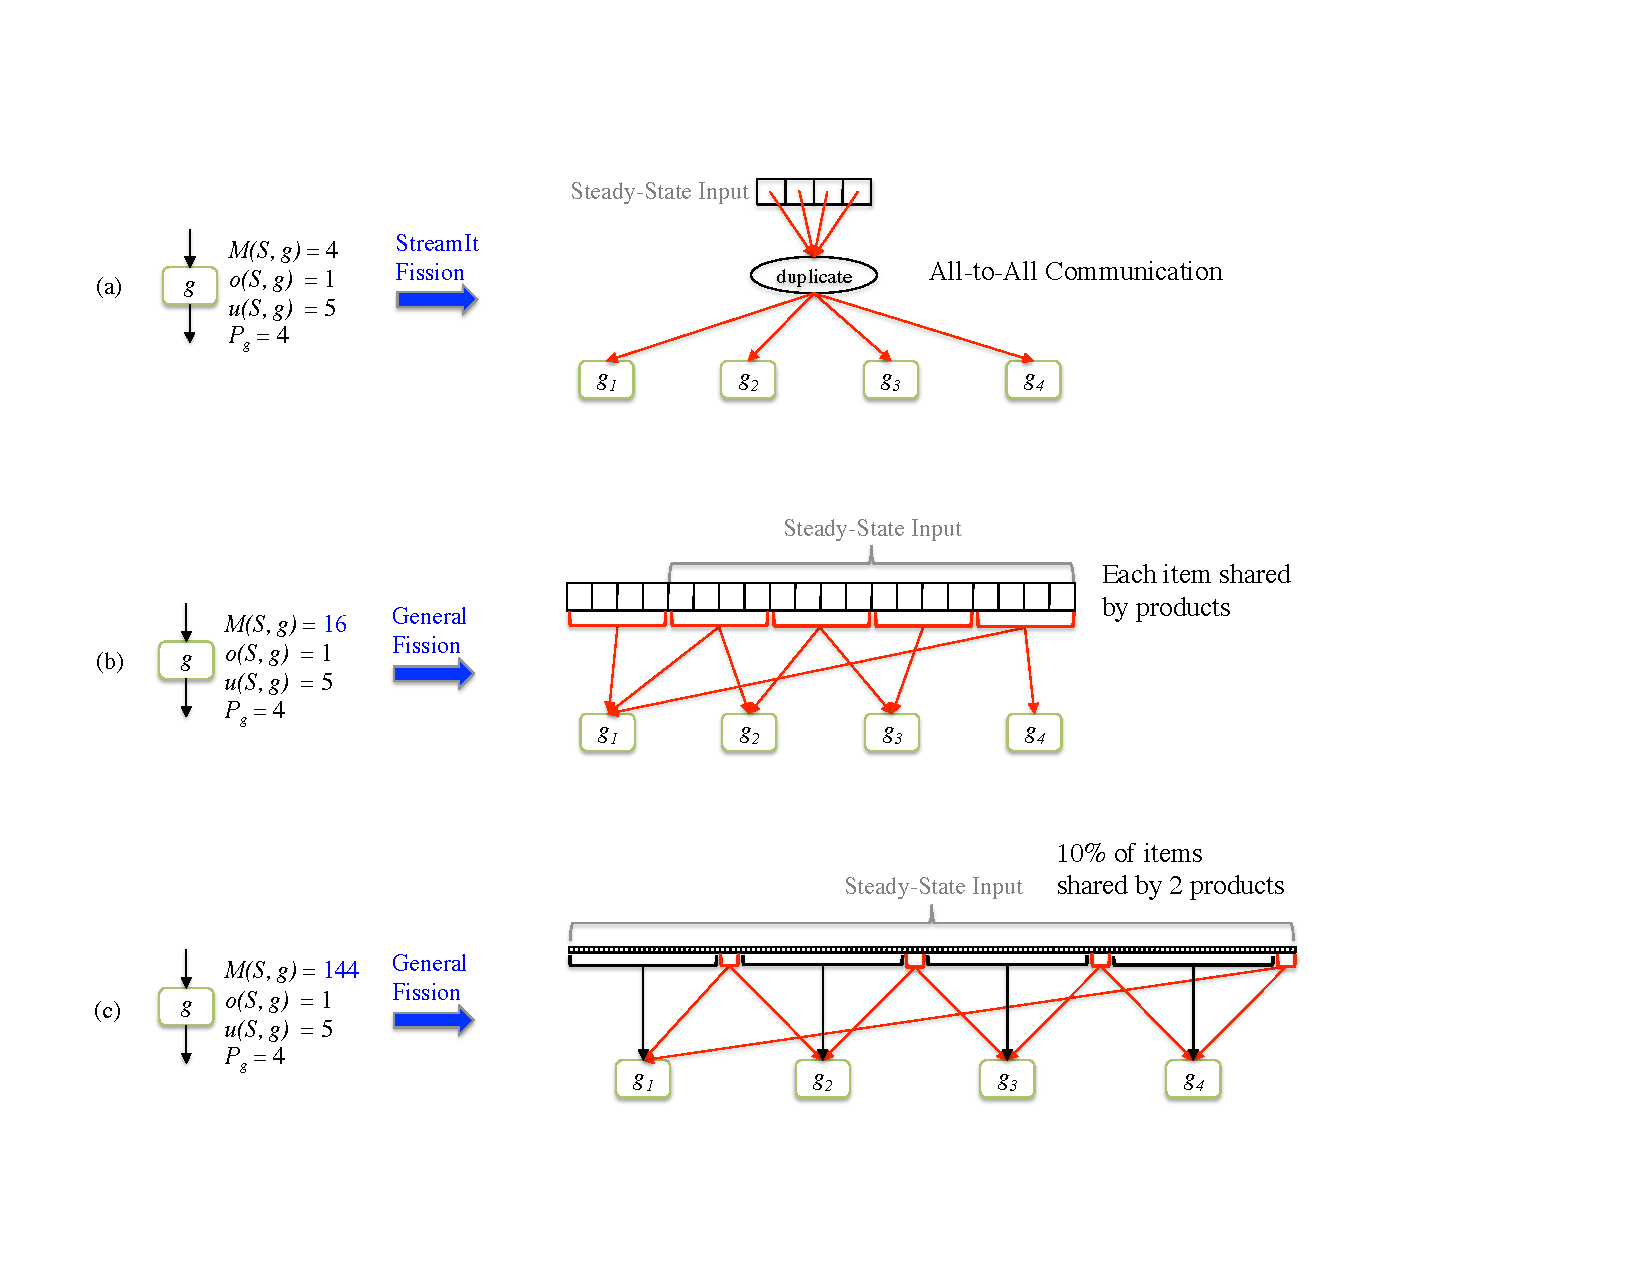
\includegraphics[width=\textwidth]{overview.pdf}
\vspace{20pt}
\caption[An overview of fission techniques.]  {
An overview of the fission techniques introduced in the paper.  The
goal of each is to fiss filter $g$ to 4 cores.  Sharing that requires
inter-core communication is denoted by red arrows. $g$ has a peek rate of
5 and a pop rate of 1.  In (a) we show the previously published fission technique
In this technique, the fission products of $g$ are placed in a splitjoin with a duplicate
splitter, and every input item is duplicated to all of the $g_i$s.
This requires all-to-all communication.  We call this technique
duplication and decimation because each input item is duplicated to
all fission products, and a fission product will decimate the item if
it does not require it.  In (b) we demonstrate our general fission, with its required steady-state alteration ($M(S, g) = 16$).  In this case the communication pattern is more efficient, and
each item is only shared by 2 fission products.  (c) demonstrates
sharing reduction.  By further increasing the steady-state
multiplicity of $g$ ($M(S, g) = 144$), we can reduce the sharing
requirement such that only 10\% of input items need to be shared by 2
fission products and 90\% input items are required by one product.
\label{fig:fission-overview}}
\end{figure}


\begin{figure}
\centering
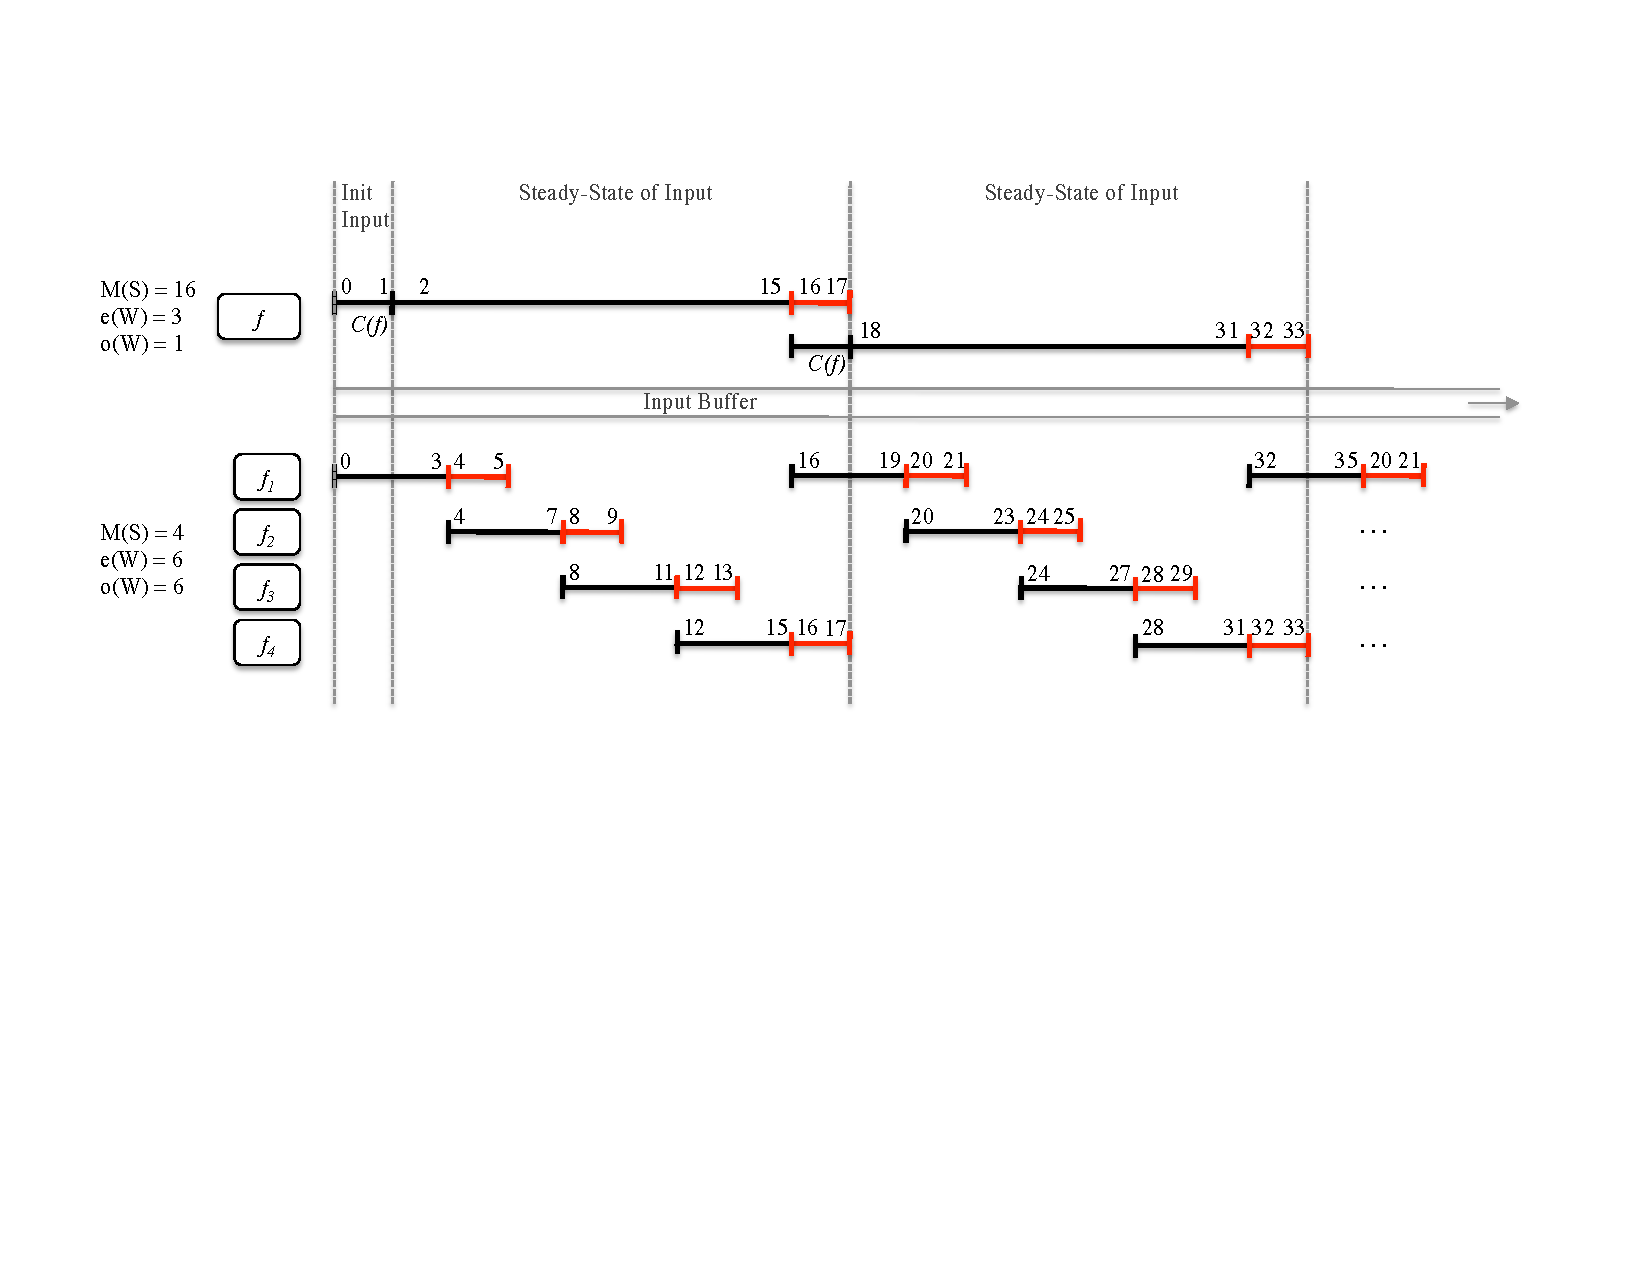
\includegraphics[width=\textwidth]{fission-sharing2.pdf}
\caption[Another example of the sharing required by fission.]  { An
  example of the sharing of items required by fission for a filter $f$
  that adheres to the preconditions for general fission.  Filter $f$
  is fissed by 4 into $f_1$ - $f_4$.  $C(f)$ items remain on the input
  buffer after initialization but before steady-state commences. Two
  steady-states of the item indices required for both $f$ and the
  fission products are shown.  Item indices that are inspected but not
  dequeued are in red.  For the fission products, it is required to
  duplicate all items to 2 filters.
  \label{fig:fission-sharing2}}
\end{figure}

\begin{figure}
\centering
\subfigure[]{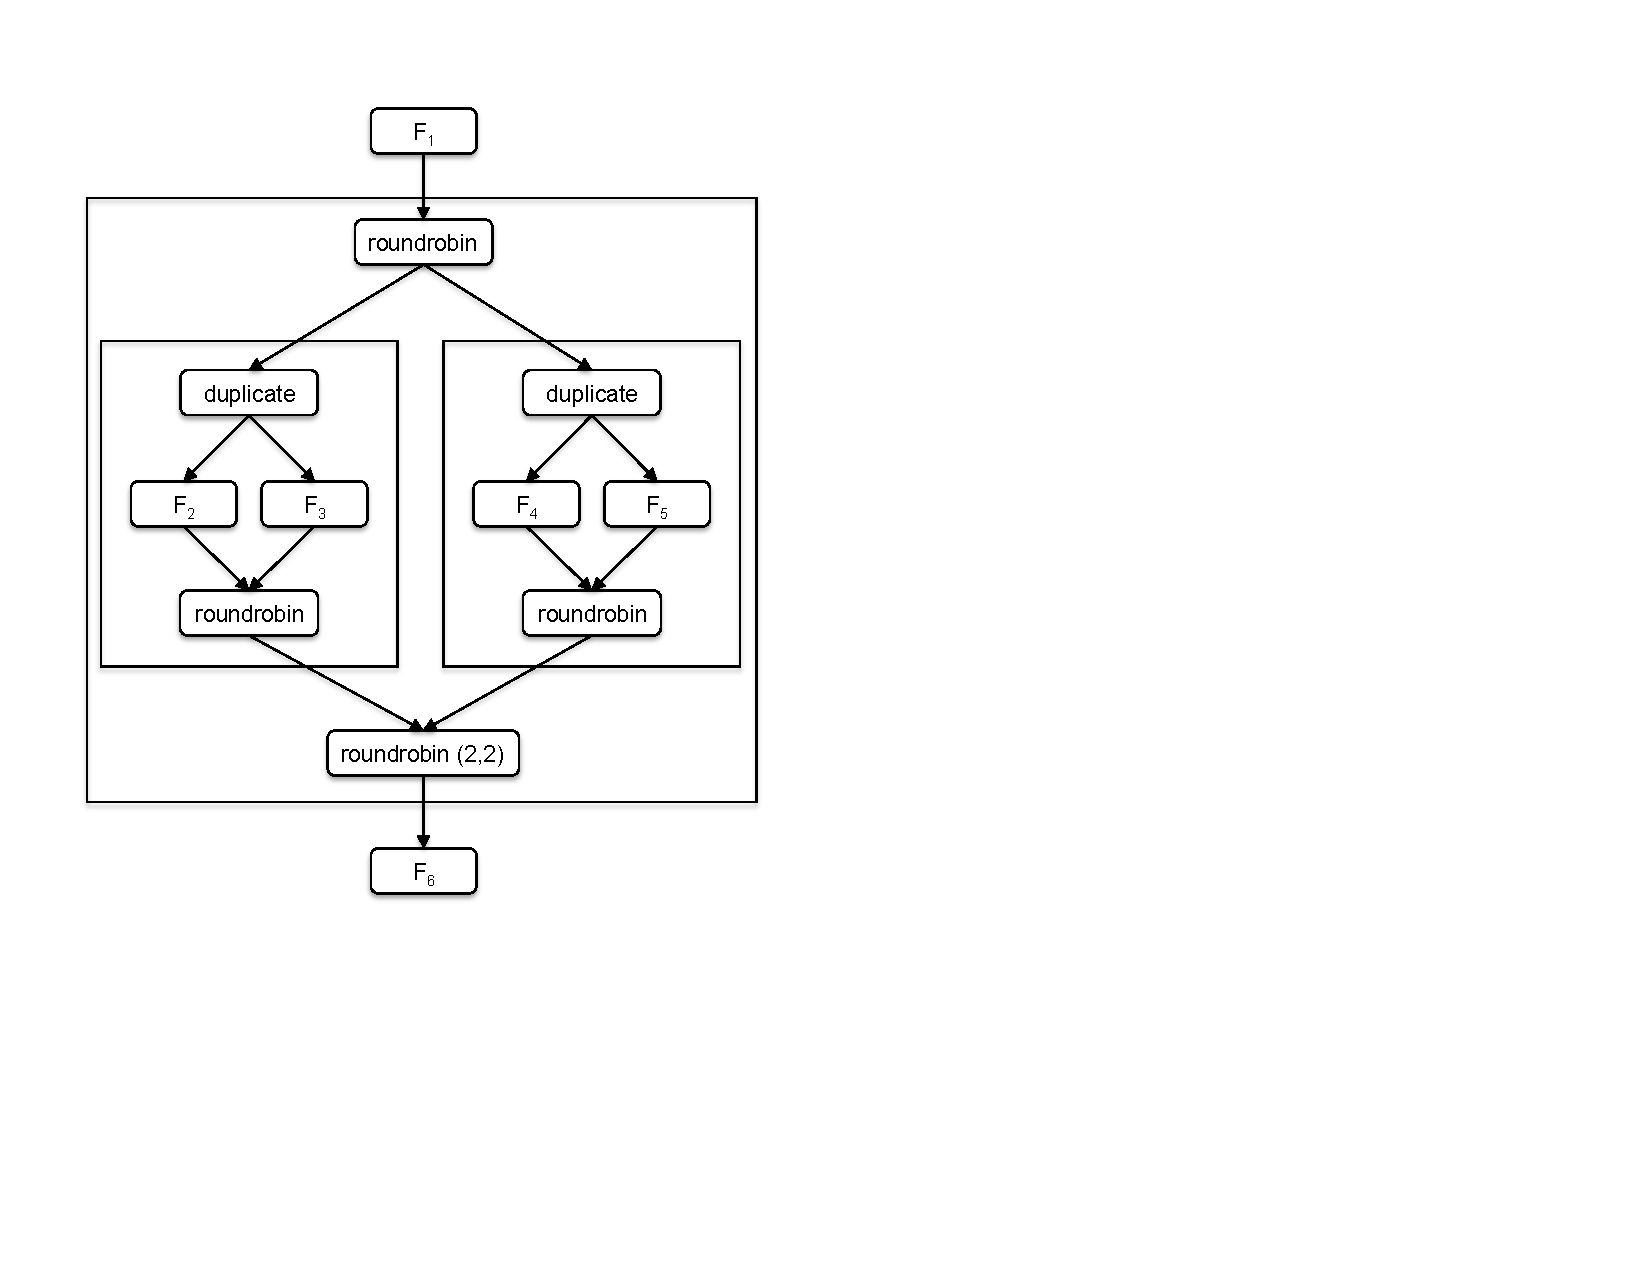
\includegraphics[width=3in]{graph-streamit.pdf}}
\qquad
\subfigure[]{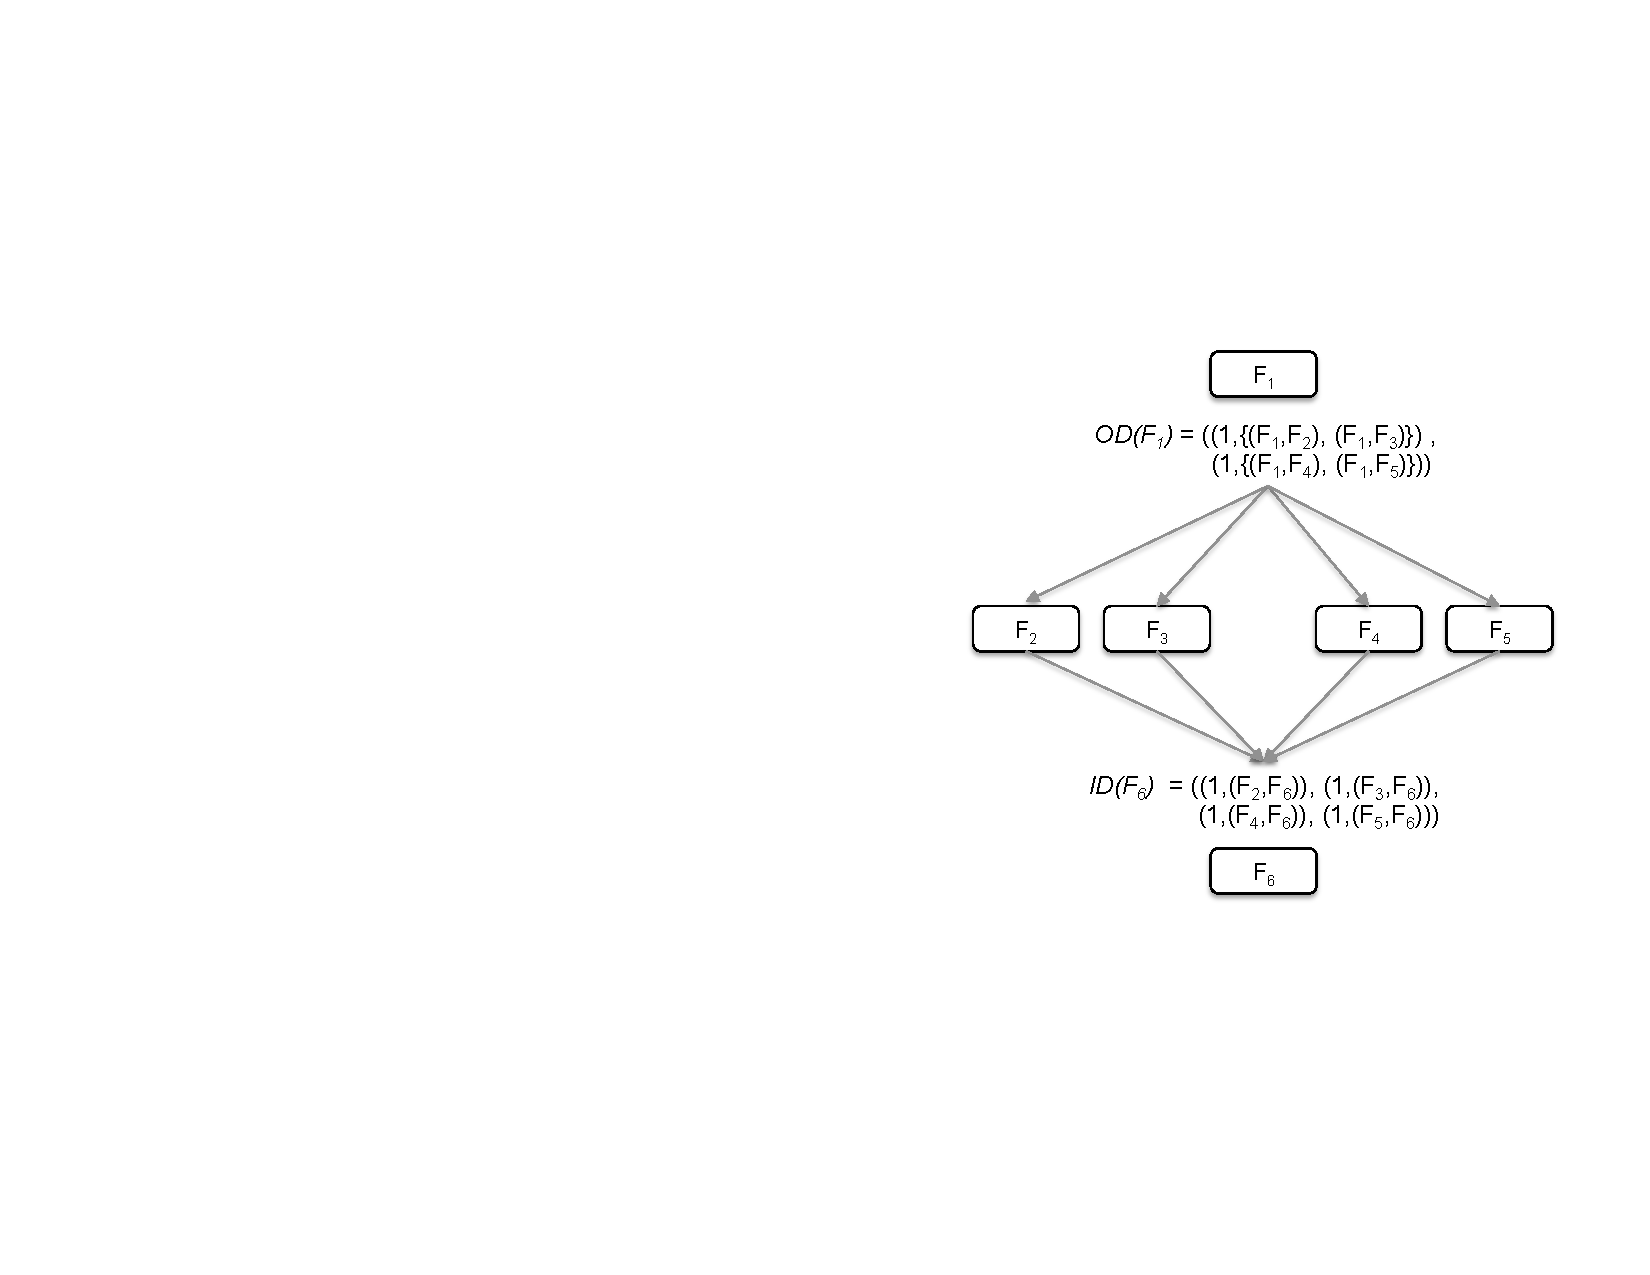
\includegraphics[width=3in]{graph-slice.pdf}}
\caption[Example of synchronization removal conversion.]{An example of
the Synchronization removal optimization.  (a) gives the original graph.  Node ``roundrobin'' and ``duplicate'' perform the identity function and exist only to distribute data.   (b) the result of removing these nodes and encoding there distribution in the remaining filters of the graph.
\label{fig:example-sr}}
\end{figure}


\begin{figure}
\centering
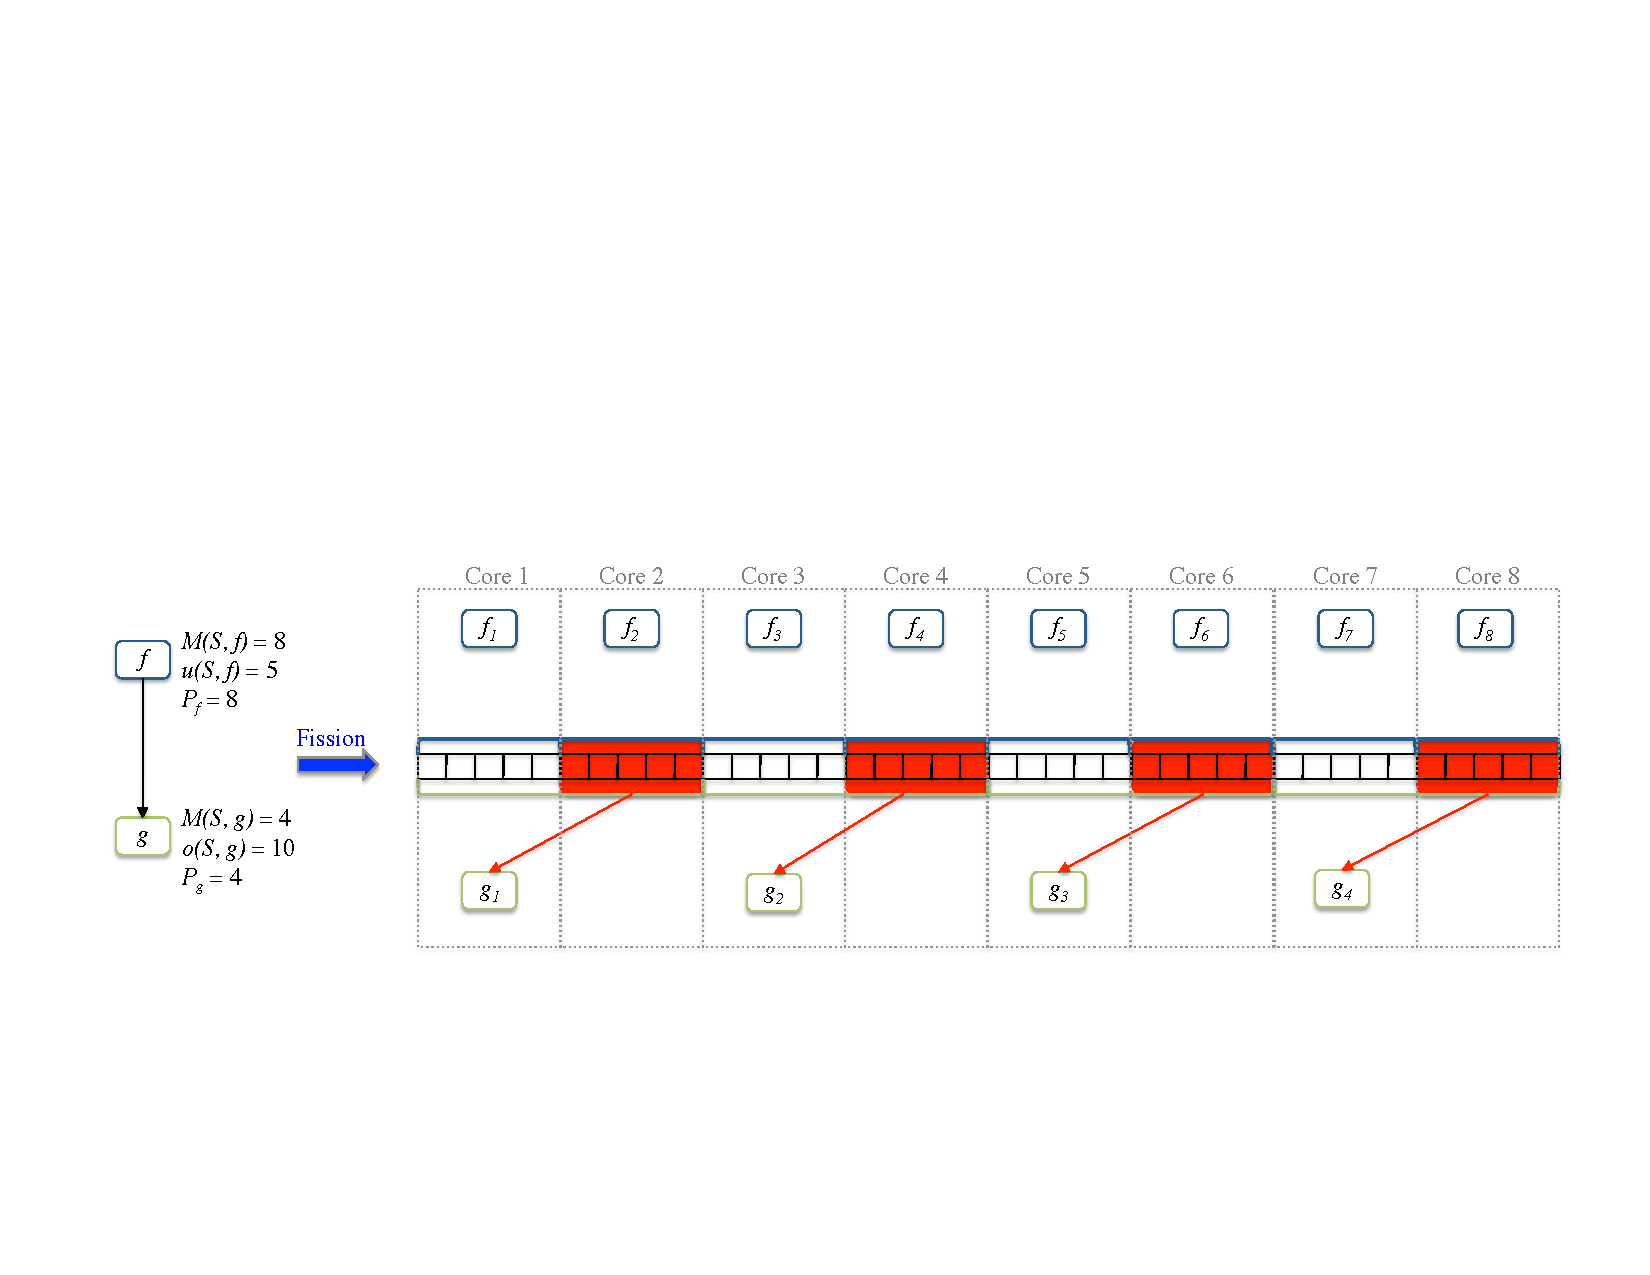
\includegraphics[width=\textwidth]{diff-widths.pdf}
\caption[Example of fission where producer fissed more than
consumer.]{An example where the producer filter $f$ is fissed by a
  greater width than the consumer filter $g$.  Assume $C(g) = 0$.  Red
  denotes inter-core communication.  Since each $f_i$ produces half
  the required input items for each $g_j$, half the communication in
  the steady-state is inter-core.  The percentage equals the ratio of
  $\frac{P_g}{P_f}$. \label{fig:diff-widths}}
\vspace{10pt}
\end{figure}


\begin{figure}
\centering
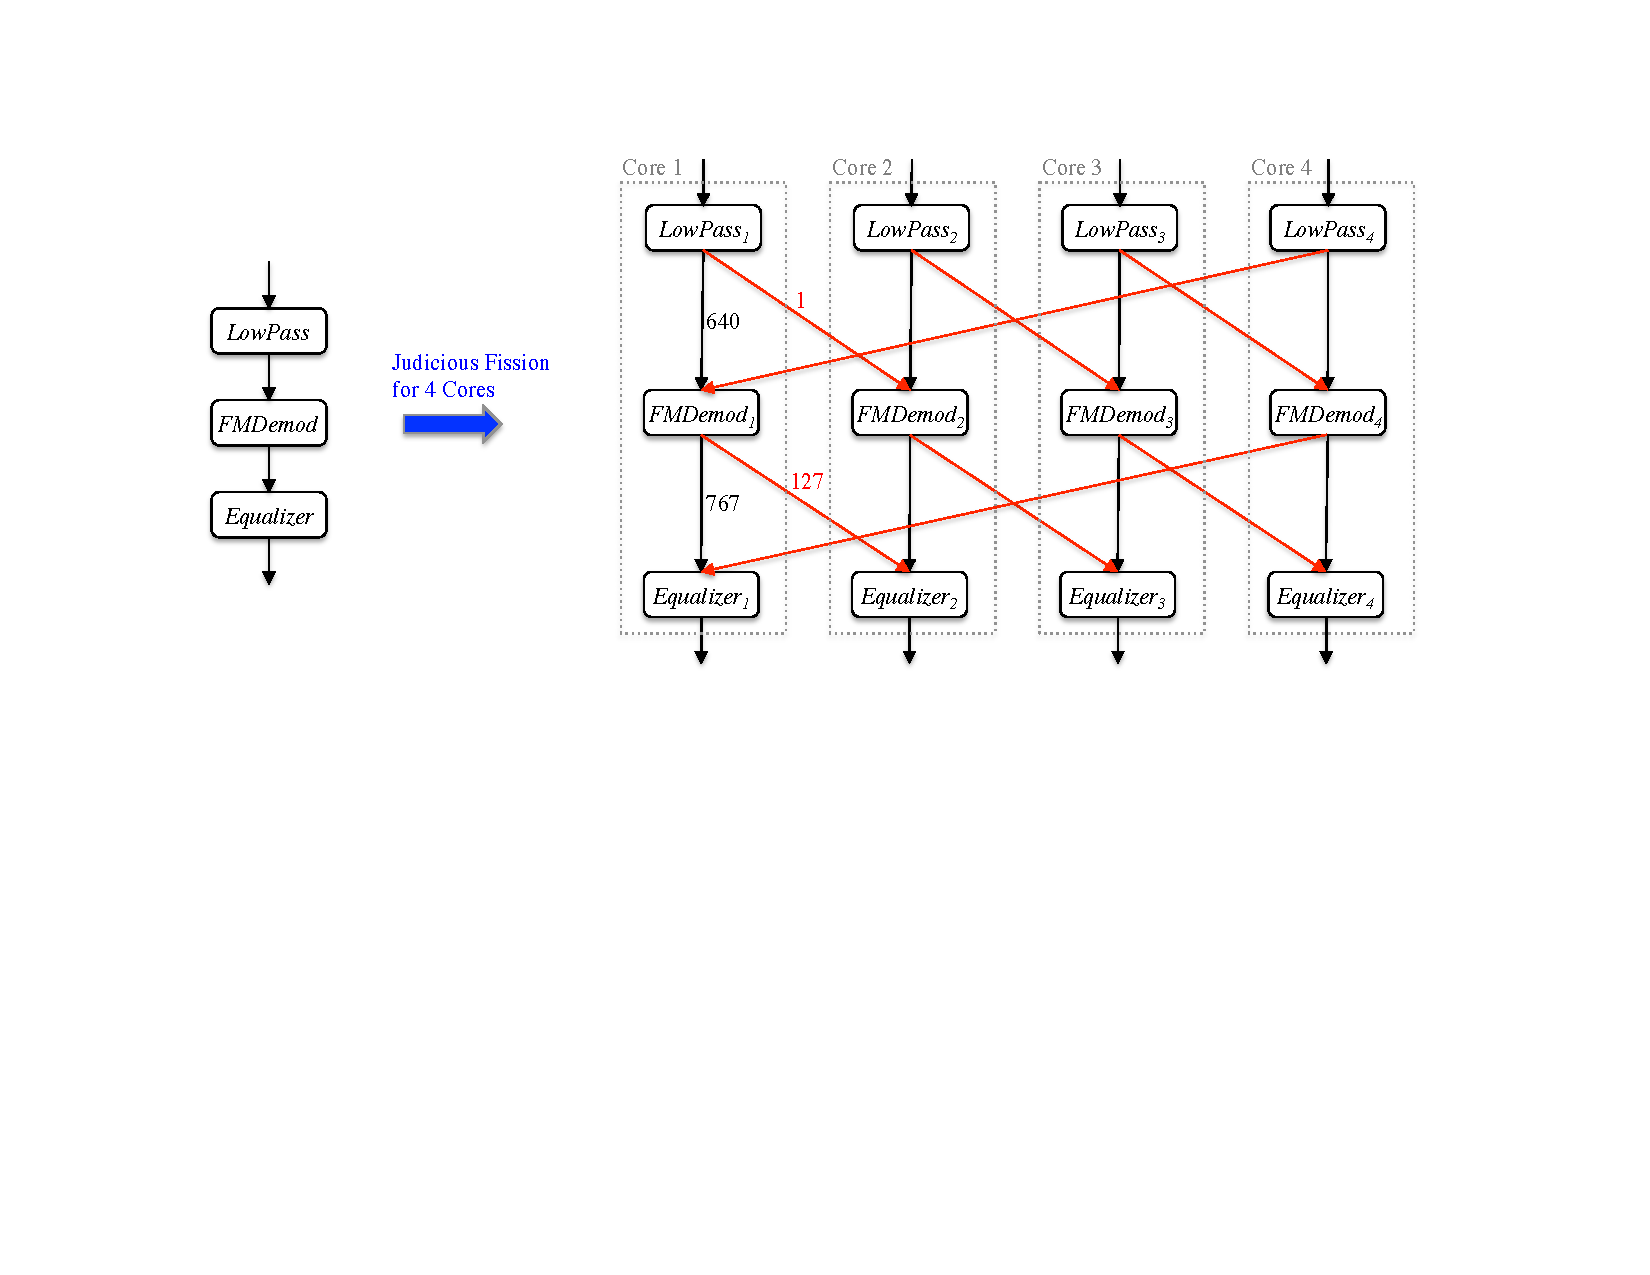
\includegraphics[width=\textwidth]{fm-4.pdf}
\caption[Judicious General Fission for FMRadio.]  { General
  fission and sharing reduction as applied to the FMRadio benchmark.  FMRadio's 
  graph is given on the left (each filter peeks).  On the right is the fissed
  result for 4 cores employing general fission. The core assignment is
  also given.  $C(f) = \mt{dup}_f$ for all filters $f$ of the
  coarsened graph.  Edges for the first core are annotated with the number
  of items communicated per steady-state.  The numbers are the same
  for the remaining cores.  Only 9\% of total non-I/O items are 
  communicated inter-core.\label{fig:fm-gen-comm}}
\end{figure}


\end{document}